\documentclass[12pt]{article}

\usepackage[margin=1in]{geometry}
\usepackage{setspace}
\onehalfspacing
\usepackage{graphicx}
\graphicspath{report_images/}
\usepackage{appendix}
\usepackage{listings}
\usepackage{float}
\usepackage{multirow}
\usepackage{amsthm}
% The next three lines make the table and figure numbers also include section number
\usepackage{chngcntr}
\counterwithin{table}{section}
\counterwithin{figure}{section}
% Needed to make titling page without a page number
\usepackage{titling}

% This section required for the code block stuff below
\usepackage{color}
\definecolor{codegreen}{rgb}{0,0.6,0}
\definecolor{codegray}{rgb}{0.5,0.5,0.5}
\definecolor{codepurple}{rgb}{0.58,0,0.82}
\definecolor{backcolour}{rgb}{0.95,0.95,0.92}

% Makes code blocks have shaded backgrounds and line numbers
\lstdefinestyle{mystyle}{
    backgroundcolor=\color{backcolour},   
    commentstyle=\color{codegreen},
    keywordstyle=\color{magenta},
    numberstyle=\tiny\color{codegray},
    stringstyle=\color{codepurple},
    basicstyle=\footnotesize,
    breakatwhitespace=false,         
    breaklines=true,                 
    captionpos=b,                    
    keepspaces=true,                 
    numbers=left,                    
    numbersep=5pt,                  
    showspaces=false,                
    showstringspaces=false,
    showtabs=false,                  
    tabsize=2
}
 
\lstset{style=mystyle}

% DOCUMENT INFORMATION =================================================
\font\titleFont=cmr12 at 11pt
\title {{\titleFont ECEN 421:  Embedded Systems Design \\ North Carolina Agricultural and Technical State University \\ Department of Electrical and Computer Engineering \\ Dr. C.A. Graves}} % Declare Title
\author{\titleFont  Chris Cannon \\ \titleFont Abbigail Waddell} % Declare authors
\date{\titleFont December 4, 2018}
% ======================================================================

\begin{document}

\begin{titlingpage}
\maketitle
\begin{center}
	Final Project Documentation
\end{center}
\end{titlingpage}

\tableofcontents

\pagebreak

\section{Introduction}
The purpose of this project is to create a design using a Texas Instruments MSP432 Launchpad and MKII Booster Pack, along with a Digilent Analog Discovery. This design should correctly identify diodes, capacitors, inductors, and resistors when these components are plugged in to our device's ports.

\section{Design Process}

\subsection{Research}
The first step in our research process was to ascertain the capabilities of the Analog Discovery. While the MSP432 was somewhat of a known quantity, neither one of us had significant experience with the Analog Discovery. Through this research, we found that the Analog Discovery had digital I/O pins and the ability to control them with JavaScript \cite{staticio} \cite{ioscript}. Once we realized that capability, we were able to quickly implement our design.

\subsection{UML Activity Diagram}

There are two basic activities taking place in our design. The first, main activity shown in Figure ~\ref{fig:mainuml} waits for the Analog Discovery to identify the component and simply displays the appropriate output on the LCD screen. The analysis subactivity shown in Figure ~\ref{fig:analuml} shows how the Analog Discovery decides what type of component it is connected to.

\begin{figure}[H]
\begin{center}
	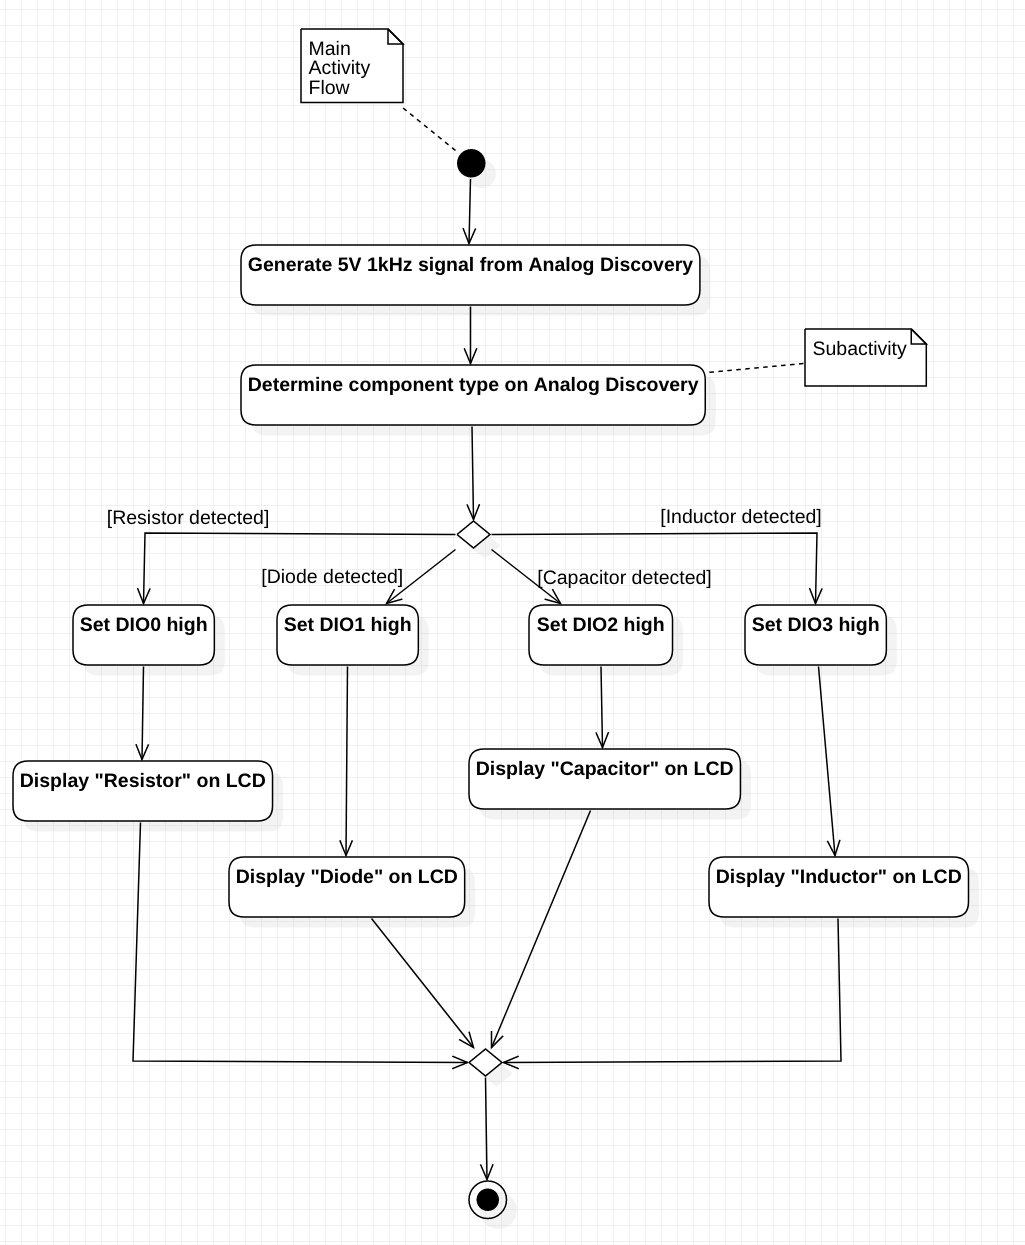
\includegraphics[width=\textwidth]{./img/MainUML.png}
	\caption{\label{fig:mainuml}IMain UML Activity Diagram}
\end{center}
\end{figure}

\begin{figure}[H]
\begin{center}
	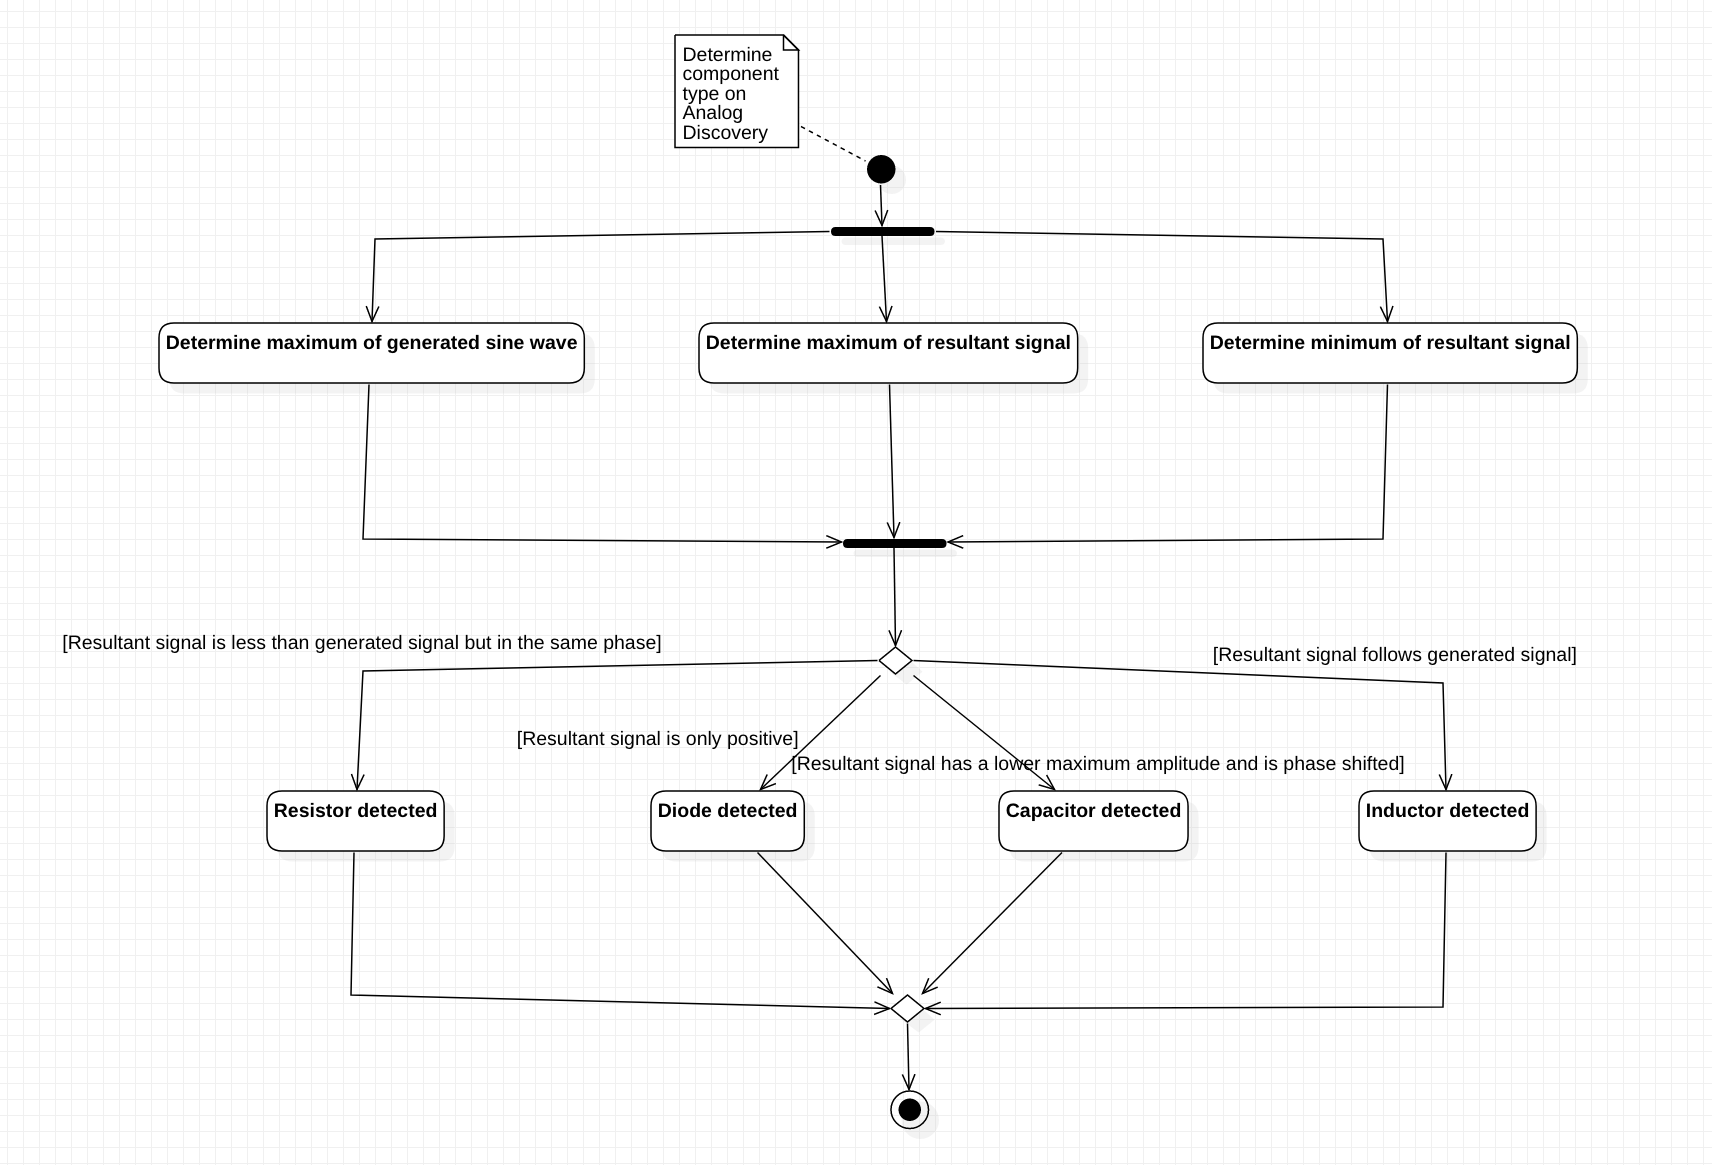
\includegraphics[width=\textwidth]{./img/AnalysisUML.png}
	\caption{\label{fig:analuml}Analysis Subactivity UML Diagram}
\end{center}
\end{figure}

\subsection{Block Diagrams}

\begin{figure}[H]
\begin{center}
	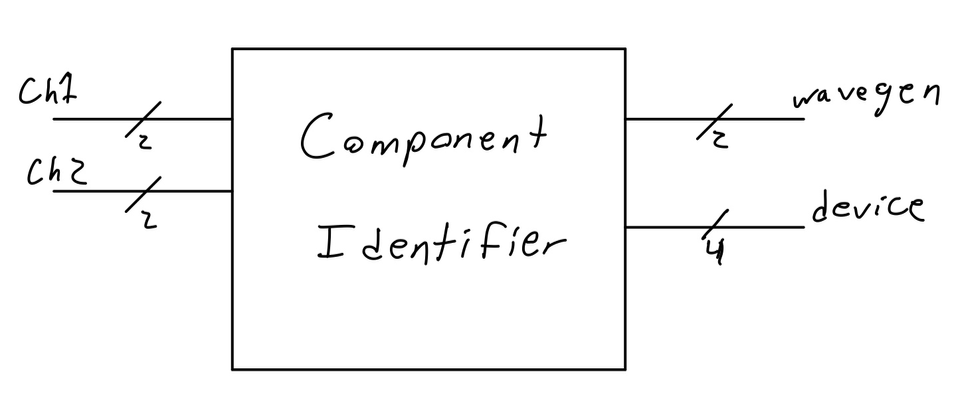
\includegraphics[width=\textwidth]{./img/level0.png}
	\caption{\label{fig:lvl0}Level 0 Block Diagram}
\end{center}
\end{figure}

\begin{figure}[H]
\begin{center}
	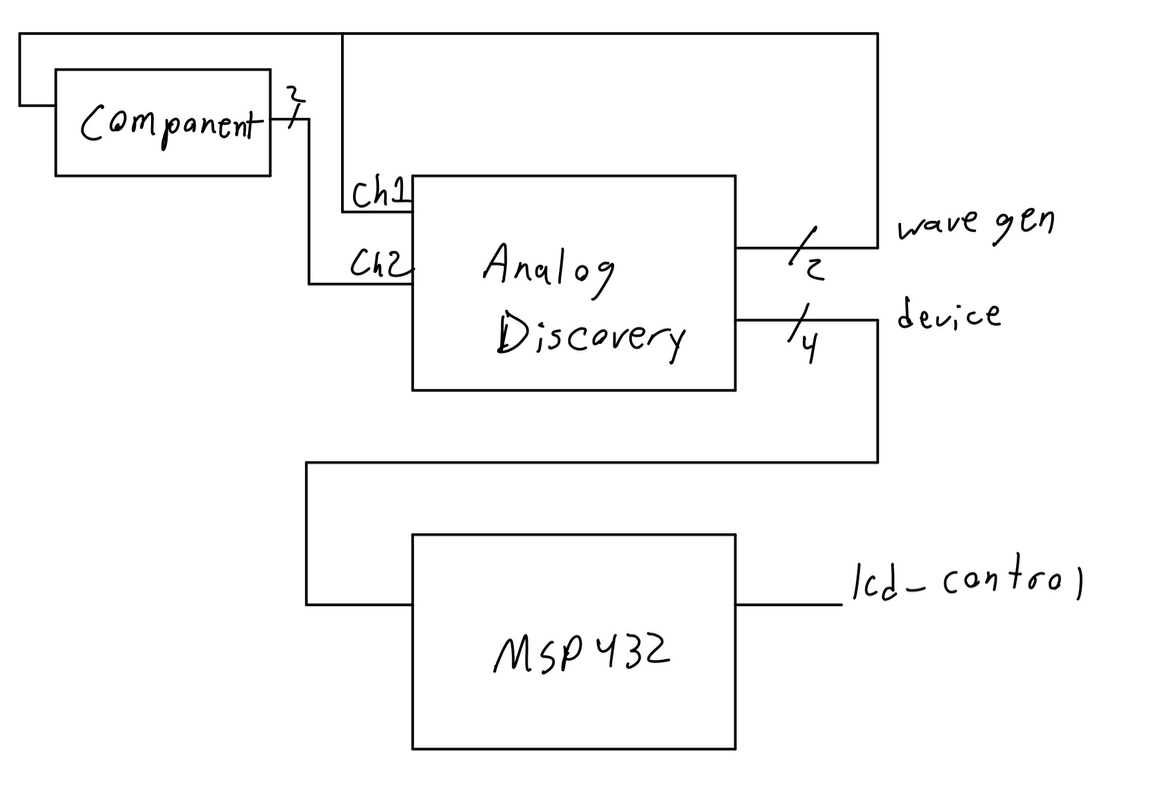
\includegraphics[width=\textwidth]{./img/level1.png}
	\caption{\label{fig:lvl1}Level 1 Block Diagram}
\end{center}
\end{figure}

\subsection{MSP432 Pin Assignments}

\begin{table}[H]
\begin{center}
\begin{tabular}{| l | l | l |}
	\hline
	\textbf{Signal Name} & \textbf{Analog Discovery Output} & \textbf{MSP432 Input} \\ \hline
	Resistor Detected Pin & DIO0 & P3.0 \\ \hline
	Diode Detected Pin & DIO1 & P3.6  \\ \hline
	Capacitor Detected Pin & DIO2 & P3.3 \\ \hline
	Inductor Detected Pin & DIO3 & P3.2  \\ \hline
\end{tabular}
\caption{\label{tab:pins}Pin assignments between the Analog Discovery and the MSP432 Launchpad}
\end{center}
\end{table}

\section{Conclusion}

With the design specified above, we were able to successfully identify diodes, resisters, inductors, and capaciters. We were able to communicate this with the MSP432 and display the output on the BoosterPack LCD screen. This project was challenging because we had to use more I/O pins than usual. This led us to researching how to control \textit{any} I/O pin, beyond the limited examples we had mostly used thus far. We were lucky to find the DriverLib functions that greatly simplified our use of input pins \cite{textbook}.

\pagebreak

\textbf{Appendices}

\begin{appendices}

\section{C Code for MSP432}

\lstinputlisting[language=C]{../main.c}

\section{JavaScript for Analog Discovery}

\lstinputlisting[language=java]{../script.js}

\end{appendices}

\begin{thebibliography}{9}

\bibitem{staticio}
  Using the Static I/O, \\
  Digilent Documentation, \\
  Digilent, Inc., \\
  \verb!https://reference.digilentinc.com/learn/instrumentation/! \\
  \verb!tutorials/ad2-static-io/start!
  
\bibitem{refman}
 Analog Discovery Technical Reference Manual, \\
 Digilent, Inc., \\
 Pullman, WA, \\
 2015 \\
 \verb![Online]! \\
 Available: \verb!https://reference.digilentinc.com/_media/! \\
 \verb!analog_discovery:analog_discovery_rm.pdf!
 
\bibitem{ioscript}
 Static IO Scripting Documents for Waveforms 3, \\
 Digilent Forums, \\
 Digilent, Inc. \\
 \verb!https://forum.digilentinc.com/topic/2150-staticio-scripting! \\
 \verb!-documentations-for-waveforms3/!
 
\bibitem{jsfunc}
 JavaScript Functions, \\
 w3schools, \\ 
 Refsnes Data, \\
 \verb!https://www.w3schools.com/js/js_functions.asp!
 
\bibitem{textbook}
 {\"U}nsalan, Cem, et al. , \\
 \textit{Programmable Microcontrollers: Applications on the MSP432 LaunchPad}, \\
 McGraw-Hill, \\
 2018
 
\end{thebibliography}
\end{document}